\documentclass[12pt,letterpaper]{article}
\usepackage{graphicx,textcomp}
\usepackage{natbib}
\usepackage{setspace}
\usepackage{fullpage}
\usepackage{color}
\usepackage[reqno]{amsmath}
\usepackage{amsthm}
\usepackage{fancyvrb}
\usepackage{amssymb,enumerate}
\usepackage[all]{xy}
\usepackage{endnotes}
\usepackage{lscape}
\newtheorem{com}{Comment}
\usepackage{float}
\usepackage{hyperref}
\newtheorem{lem} {Lemma}
\newtheorem{prop}{Proposition}
\newtheorem{thm}{Theorem}
\newtheorem{defn}{Definition}
\newtheorem{cor}{Corollary}
\newtheorem{obs}{Observation}
\usepackage[compact]{titlesec}
\usepackage{dcolumn}
\usepackage{tikz}
\usetikzlibrary{arrows}
\usepackage{multirow}
\usepackage{xcolor}
\newcolumntype{.}{D{.}{.}{-1}}
\newcolumntype{d}[1]{D{.}{.}{#1}}
\definecolor{light-gray}{gray}{0.65}
\usepackage{url}
\usepackage{listings}
\usepackage{color}

\definecolor{codegreen}{rgb}{0,0.6,0}
\definecolor{codegray}{rgb}{0.5,0.5,0.5}
\definecolor{codepurple}{rgb}{0.58,0,0.82}
\definecolor{backcolour}{rgb}{0.95,0.95,0.92}

\lstdefinestyle{mystyle}{
	backgroundcolor=\color{backcolour},   
	commentstyle=\color{codegreen},
	keywordstyle=\color{magenta},
	numberstyle=\tiny\color{codegray},
	stringstyle=\color{codepurple},
	basicstyle=\footnotesize,
	breakatwhitespace=false,         
	breaklines=true,                 
	captionpos=b,                    
	keepspaces=true,                 
	numbers=left,                    
	numbersep=5pt,                  
	showspaces=false,                
	showstringspaces=false,
	showtabs=false,                  
	tabsize=2
}
\lstset{style=mystyle}
\newcommand{\Sref}[1]{Section~\ref{#1}}
\newtheorem{hyp}{Hypothesis}

\title{Problem Set 3}
\date{Due: November 20, 2022}
\author{Applied Stats/Quant Methods 1}


\begin{document}
	\maketitle
	\section*{Instructions}
	\begin{itemize}
		\item Please show your work! You may lose points by simply writing in the answer. If the problem requires you to execute commands in \texttt{R}, please include the code you used to get your answers. Please also include the \texttt{.R} file that contains your code. If you are not sure if work needs to be shown for a particular problem, please ask.
	\item Your homework should be submitted electronically on GitHub.
	\item This problem set is due before 23:59 on Sunday November 20, 2022. No late assignments will be accepted.
	\item Total available points for this homework is 80.
	\end{itemize}

		\vspace{.25cm}
	
\noindent In this problem set, you will run several regressions and create an add variable plot (see the lecture slides) in \texttt{R} using the \texttt{incumbents\_subset.csv} dataset. Include all of your code.

	\vspace{.5cm}
\section*{Question 1}
\vspace{.25cm}
\noindent We are interested in knowing how the difference in campaign spending between incumbent and challenger affects the incumbent's vote share. 
	\begin{enumerate}
		\item Run a regression where the outcome variable is \texttt{voteshare} and the explanatory variable is \texttt{difflog}.	
		
		First I load the data into my R Studio session using the below code:
		\lstinputlisting[language=R, firstline=34, lastline=34]{PS3.R} 
		
		Then I run the regression with the following code:
		\lstinputlisting[language=R, firstline=41, lastline=41]{PS3.R} 
			\begin{figure}
			\begin{verbatim}
				Residuals:     Min       1Q   Median       3Q      Max
				 -0.26832 -0.05345 -0.00377  0.04780  0.32749 
				 Coefficients:            
				             Estimate    Std. Error  t value Pr(>|t|)
				 (Intercept) 0.579031   0.002251  257.19   <2e-16 ***
				 difflog     0.041666   0.000968   43.04   <2e-16 ***
				 ---
				 Signif. codes:  0 ‘***’ 0.001 ‘**’ 0.01 ‘*’ 0.05 ‘.’ 0.1 ‘ ’ 1
				 Residual standard error: 0.07867 on 3191 degrees of freedom
				 Multiple R-squared:  0.3673,	Adjusted R-squared:  0.3671 
				 F-statistic:  1853 on 1 and 3191 DF,  p-value: < 2.2e-16
			\end{verbatim}
		
		\end{figure}
		
		\vspace{5cm}
		\item Make a scatterplot of the two variables and add the regression line. 
		
		First I made the scatterplot (with x = difflog, y = voteshare) using the following code:
		\lstinputlisting[language=R, firstline=49, lastline=51]{PS3.R} 
		
		The scatterplot is below:
		\begin{center}	
			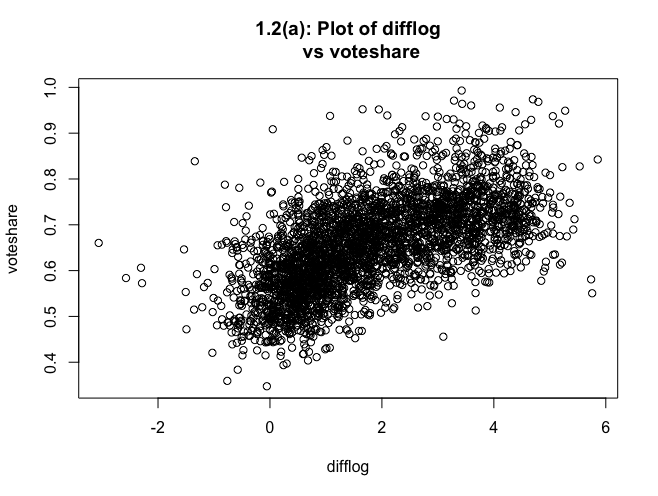
\includegraphics[scale=.80]{Plot1.2(a).png}
		\end{center}
		
		Then I added the Regression Line to this plot with the following code:
		\lstinputlisting[language=R, firstline=55, lastline=59]{PS3.R} 
		Which produced the following plot:
		\begin{center}	
		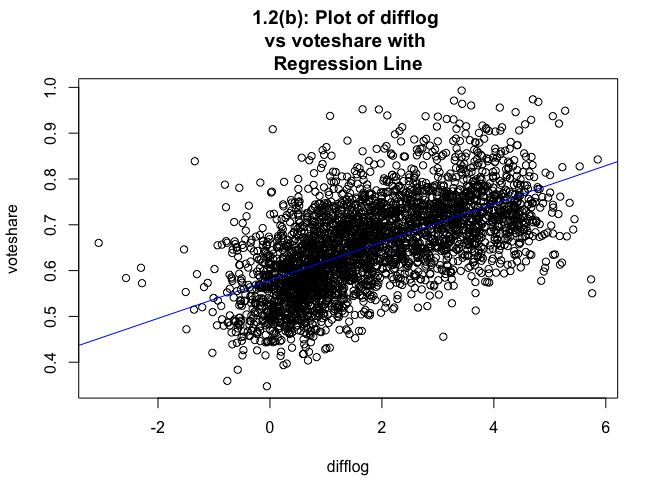
\includegraphics[scale=.80]{Plot1.2(b).png}
		\end{center}
		
			\vspace{1cm}
		\item Save the residuals of the model in a separate object.
		I do this with the following code:
		\lstinputlisting[language=R, firstline=65, lastline=65]{PS3.R} 
		
			\vspace{7cm}
		\item Write the prediction equation.
		
		y hat = intercept + slope*x
		
		Predicted voteshare = 0.579 + 0.042(difflog)
	\end{enumerate}
	
\newpage

\section*{Question 2}
\noindent We are interested in knowing how the difference between incumbent and challenger's spending and the vote share of the presidential candidate of the incumbent's party are related.	\vspace{.25cm}
	\begin{enumerate}
		\item Run a regression where the outcome variable is \texttt{presvote} and the explanatory variable is \texttt{difflog}.
		
		Code for regression with outcome variable presvote, explanatory variable:
		\lstinputlisting[language=R, firstline=75, lastline=75]{PS3.R}
		Summary of this regression output is below:
		
			\begin{verbatim}
		Residuals:     Min       1Q   Median       3Q      Max 
		-0.32196 -0.07407 -0.00102  0.07151  0.42743
		 Coefficients:  
		           Estimate Std. Error t value Pr(>|t|)
    (Intercept) 0.507583   0.003161  160.60   <2e-16 ***
    difflog     0.023837   0.001359   17.54   <2e-16 ***
    ---
    Signif. codes:  0 ‘***’ 0.001 ‘**’ 0.01 ‘*’ 0.05 ‘.’ 0.1 ‘ ’ 1
    Residual standard error: 0.1104 on 3191 degrees of freedom
    Multiple R-squared:  0.08795,	Adjusted R-squared:  0.08767 
    F-statistic: 307.7 on 1 and 3191 DF,  p-value: < 2.2e-16
		\end{verbatim} 
		
			\vspace{2cm}
		\item Make a scatterplot of the two variables and add the regression line. 
		
To first plot the two variables I input the following code:
	\lstinputlisting[language=R, firstline=81, lastline=83]{PS3.R}
	
The plot of these two variables is below:

	\begin{center}	
		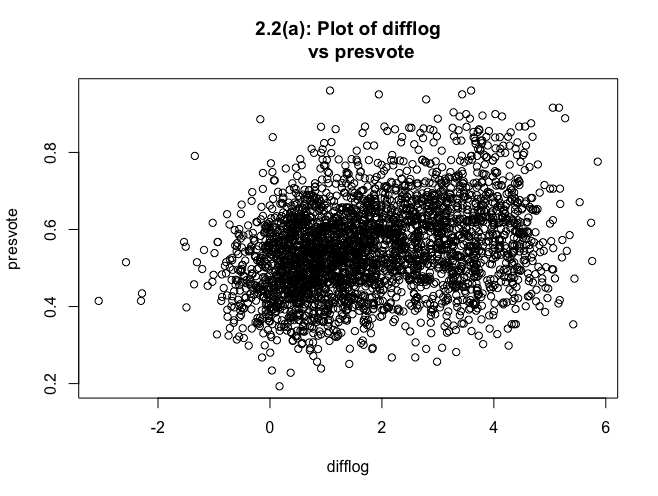
\includegraphics[scale=.80]{Plot2.2(a).png}		\end{center}
	
Then I added the regression line with the following code:

	\lstinputlisting[language=R, firstline=87, lastline=91]{PS3.R}

The plot produced with the regression line included is below:
	\begin{center}	
	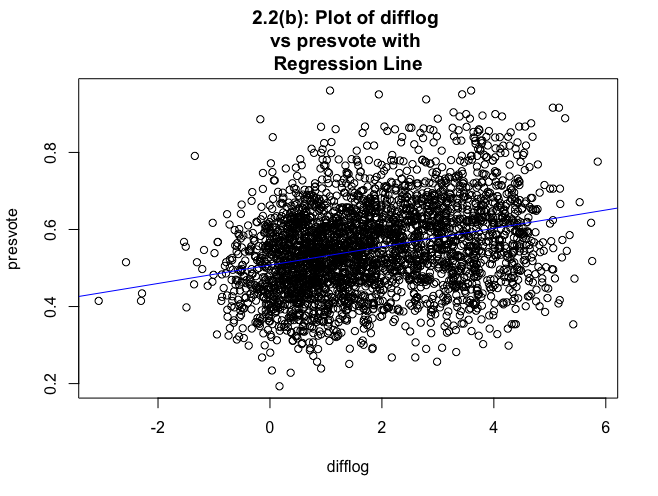
\includegraphics[scale=.80]{Plot2.2(b).png}		\end{center}	
		
			\vspace{2cm}
		\item Save the residuals of the model in a separate object.
I did this with the following code:
	\lstinputlisting[language=R, firstline=97, lastline=97]{PS3.R}
			
			\vspace{1cm}
		\item Write the prediction equation.

y hat = intercept + slope*x

Predicted presvote = 0.508 + 0.024(difflog)		

	\end{enumerate}
	
	\newpage	
\section*{Question 3}

\noindent We are interested in knowing how the vote share of the presidential candidate of the incumbent's party is associated with the incumbent's electoral success.
	\vspace{.25cm}
	\begin{enumerate}
		\item Run a regression where the outcome variable is \texttt{voteshare} and the explanatory variable is \texttt{presvote}.
		
Regression run with those variables with the below code:
	\lstinputlisting[language=R, firstline=105, lastline=105]{PS3.R}
	
Summary output of this regression:
			\begin{verbatim}
Residuals:     Min       1Q   Median       3Q      Max 
-0.27330 -0.05888  0.00394  0.06148  0.41365 
Coefficients:            
		Estimate Std. Error t value Pr(>|t|)
(Intercept) 0.441330   0.007599   58.08   <2e-16
presvote    0.388018   0.013493   28.76   <2e-16               
(Intercept) ***
presvote    ***
---
Signif. codes:  0 ‘***’ 0.001 ‘**’ 0.01 ‘*’ 0.05 ‘.’ 0.1 ‘ ’ 1
Residual standard error: 0.08815 on 3191 degrees of freedom
Multiple R-squared:  0.2058,	Adjusted R-squared:  0.2056 
F-statistic:   827 on 1 and 3191 DF,  p-value: < 2.2e-16
\end{verbatim} 

			\vspace{2cm}
		\item Make a scatterplot of the two variables and add the regression line.

I plot the two variables using the following code:
\lstinputlisting[language=R, firstline=112, lastline=114]{PS3.R}	
The plot of these two variables is below:

\begin{center}	
	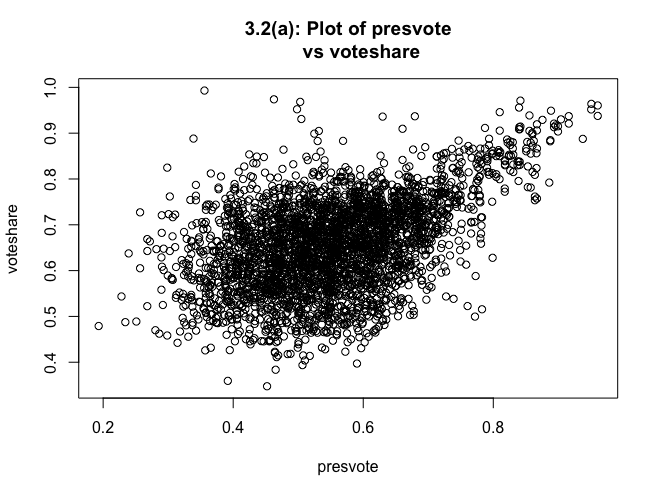
\includegraphics[scale=.80]{Plot3.2(a).png}		\end{center}

Then I added the regression line with the following code:

\lstinputlisting[language=R, firstline=118, lastline=122]{PS3.R}

The plot produced with the regression line included is below:
\begin{center}	
	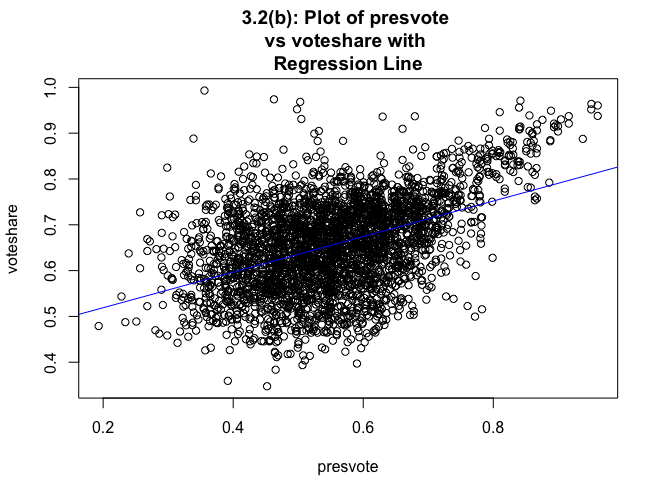
\includegraphics[scale=.80]{Plot3.2(b).png}		\end{center}	
 
		\vspace{2cm}
		\item Write the prediction equation.

y hat = intercept + slope*x

Predicted voteshare = 0.441 + 0.388(presvote)		
		
	\end{enumerate}
	

\newpage	
\section*{Question 4}
\noindent The residuals from part (a) tell us how much of the variation in \texttt{voteshare} is $not$ explained by the difference in spending between incumbent and challenger. The residuals in part (b) tell us how much of the variation in \texttt{presvote} is $not$ explained by the difference in spending between incumbent and challenger in the district.
	\begin{enumerate}
		\item Run a regression where the outcome variable is the residuals from Question 1 and the explanatory variable is the residuals from Question 2.
		
To run this regression I input the following code:
\lstinputlisting[language=R, firstline=128, lastline=128]{PS3.R}

Which output the following regression summary:

			\begin{verbatim}
Residuals:
     Min       1Q   Median       3Q      Max
 -0.25928 -0.04737 -0.00121  0.04618  0.33126
  Coefficients:               
               Estimate Std. Error t value Pr(>|t|)    
  (Intercept)  -4.860e-18  1.299e-03    0.00        1    
  Res_lm_pv_dl  2.569e-01  1.176e-02   21.84   <2e-16 ***
  ---
  Signif. codes:  0 ‘***’ 0.001 ‘**’ 0.01 ‘*’ 0.05 ‘.’ 0.1 ‘ ’ 1
  Residual standard error: 0.07338 on 3191 degrees of freedom
  Multiple R-squared:   0.13,	Adjusted R-squared:  0.1298 
  F-statistic:   477 on 1 and 3191 DF,  p-value: < 2.2e-16				
\end{verbatim} 		
			\vspace{2cm}
		\item Make a scatterplot of the two residuals and add the regression line.
I make the scatterplot with the following code:
\lstinputlisting[language=R, firstline=133, lastline=135]{PS3.R}

This produces the scatterplot below:
\begin{center}	
	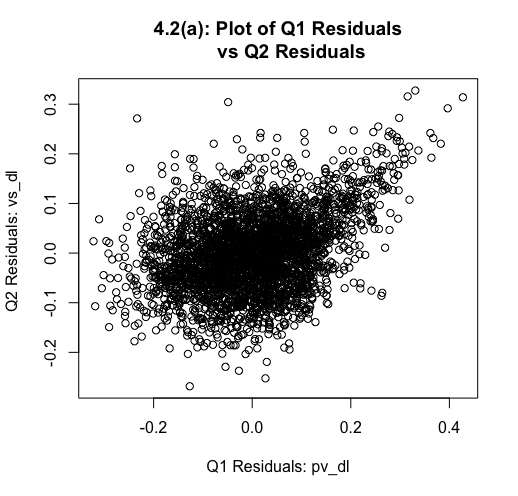
\includegraphics[scale=.80]{Plot4.2(a).png}		\end{center}


I add the regression line with the following code:
\lstinputlisting[language=R, firstline=137, lastline=140]{PS3.R}

This produces the scatterplot plus regression line below:		
\begin{center}	
	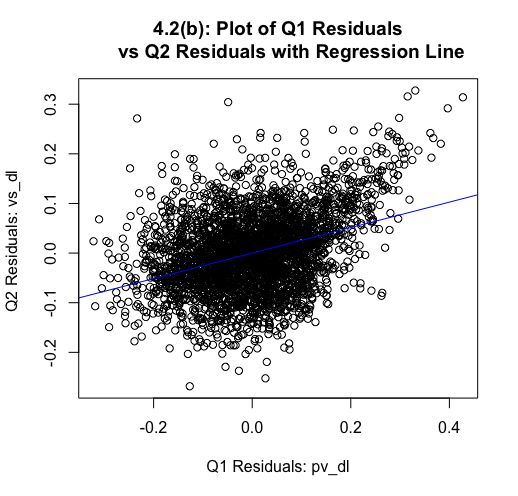
\includegraphics[scale=.80]{Plot4.2(b).png}		\end{center}
		
		 	\vspace{2cm}
		\item Write the prediction equation.
		
The prediction equation is:
y hat = intercept + slope*x

(Amount of variation in vote share not explained by the diff in spending between the incumbent and challenger) = -4.860e-18 + 2.569e-1(variation in presvote not explained by the difference in spending between the incumbent and challenger)		

	\end{enumerate}
	
	\newpage	

\section*{Question 5}
\noindent What if the incumbent's vote share is affected by both the president's popularity and the difference in spending between incumbent and challenger? 
	\begin{enumerate}
		\item Run a regression where the outcome variable is the incumbent's \texttt{voteshare} and the explanatory variables are \texttt{difflog} and \texttt{presvote}.
To run this regression I input the following code:
\lstinputlisting[language=R, firstline=146, lastline=146]{PS3.R}
Which results in this output:
	\begin{verbatim}
Residuals:     
Min       1Q   Median       3Q      Max 
-0.25928 -0.04737 -0.00121  0.04618  0.33126 
Coefficients:             
          	Estimate Std. Error t value Pr(>|t|)
(Intercept) 0.4486442  0.0063297   70.88   <2e-16
difflog     0.0355431  0.0009455   37.59   <2e-16
presvote    0.2568770  0.0117637   21.84   <2e-16               
(Intercept) ***
difflog     ***
presvote    ***
---
Signif. codes:  0 ‘***’ 0.001 ‘**’ 0.01 ‘*’ 0.05 ‘.’ 0.1 ‘ ’ 1
Residual standard error: 0.07339 on 3190 degrees of freedom
Multiple R-squared:  0.4496,	Adjusted R-squared:  0.4493 
F-statistic:  1303 on 2 and 3190 DF,  p-value: < 2.2e-16		
\end{verbatim} 				
		
		
			\vspace{2cm}
		\item Write the prediction equation.	
Prediction equation is:
The prediction equation is:
y hat = intercept + slope*x

(predicted voteshare) = 0.449 + 0.036(difflog) + 0.257(presvote)			
		
\vspace{5cm}
		\item What is it in this output that is identical to the output in Question 4? Why do you think this is the case?

The residuals are identical in this output and that of Question 4. This is because Question 4 runs a regression that's output shows how much that variation in voteshare not explained by difflog is explained by the variation in presvote that is also not explained by difflog. Then, when the residuals are taken from this Question 4 output, these residuals show how much of the voteshare variation is NOT explained both by difflog and presvote. 
Then, the additive linear regression model ran in Question 5 shows how much  variation in voteshare is explained by the difflog plus presvote variables. Thus, the residuals of this regression model (from Question 5) are essentially showing the same thing as the residuals in Question 4: the variation in voteshare that is NOT explained by both difflog and presvote. Essentially, these residuals were obtained by running regressions of two different models, can be interpreted as showing the same thing.
	\end{enumerate}




\end{document}
